\chapter{特征表示的底层语义应用}
\label{chap:Denoising}


\section{图像的去噪方法}
图像去噪的目的是从噪声图像中恢复出干净的图像,这是低级视觉任务中的一个经典问题。由于无噪声的原图像通常是未知的,因此这个问题本质上是不适定的,即它是一个欠定的映射问题,通常映射变换不唯一。一般来说,残差图像$ F $可以表示为$ F = y-f(x)$,其中$ x $是噪声图像,$ f $是映射函数,它接收输入图像并将其转换为输出图像。$ y $是理想的无噪声图像。通过应用不同类型的映射函数,相同的数学模型适用于大多数其他低层级的视觉图像任务,如图像去模糊,去马赛克和超分辨率等。

最近,无论是从高级到低级任务,深度神经网络在计算机视觉领域表现出了卓越的性能。众所周知,神经网络能够将任何可测量的函数逼近到期望的准确度\cite{Hornik1989}。在图像去噪场景下,回归框架中的神经网络试图在某些输入噪声分布下逼近潜在条件期望。当以监督方式训练前馈神经网络时,一个关键因素是选择损失函数来测量输出和真实图像之间的差异。最广泛使用的是像素损失,其通过失真和参考图像像素的强度差异以及相关的峰值信噪比\cite{Wang2004}来计算。但是,像素损失不能捕捉到感知差异,并且与人类感知图像质量的关联性很差\cite{Zhao2015,Zhanga2012}。这是因为当使用像素损失时隐含地做出的许多假设不能被满足-其主要仅依据独立于图像的局部灰度特征来处理噪声;相反,人类视觉系统对噪声的敏感性取决于局部亮度,对比度和结构等综合因素\citep{Wang2004}。

基于纯粹的学习策略,为图像去噪设计的一组深度神经网络已被证明优于其他被广泛采用的方法\cite{Burger2012}。但是,所有这些工作都存在一个问题:如果输入无噪图像,则学习到的模型仍会降低并没噪声的原图像的质量。所以他们工作就是必须限定在给定噪声水平下才有效。用于去噪声的通用标准算法应该能够处理不同级别的噪声,针对具体不同噪声水平需要一系列这样的网络,这是不切实际的,甚至是不现实的。因为我们不知道真实图像具体的噪声水平和类型。

我们的主要贡献简要概述如下:
\begin{enumerate}
\item 我们提出了一个较深的全卷积网络结构,用于图像残差去噪。针对图像变换对残差映射函数进行建模,直接学习噪声分布。
\item 结合每像素和感知丢失函数的优点,训练具有低和高级别信息的转换网络,生成高质量的去噪图像。
\item 为使单个神经网络适用于所有噪声级别,我们研究网络的统计规律:使输入从不同噪声级别添加随机样本,输入也可以是干净的图像,因为学习的图像函数必须对干净的图像进行身份验证,训练有素的网络可以自动处理不同的级别。
\item 我们试验了一些常见的基准图像。结果表明我们的网络的优点和所提出的新型损失层克服了其他最近的图像去噪方面的最新技术方法。
\end{enumerate}

\subsection{相关工作}
已经提出了许多用于图像去噪的方法。一些有选择地平滑噪声图像的部分,目的是在保留图像细节的同时“平滑”噪声。一些方法将图像信号传送到可以容易地从信号中分离噪声的替代域。最近的方法利用图像的“非本地”统计:相同图像中的不同补丁在外观上通常相似。块匹配和3D过滤(BM3D)算法\cite{Dabov2007}通过协作过滤在变换域中对非局部相似补丁进行分组。BM3D已经成为图像去噪的基准。

虽然BM3D是一种设计良好的算法,但基于学习的方法已经广泛用于图像去噪。神经网络方法和其他方法最显着的区别在于,它们通常自动直接从干净而嘈杂的图像中自动学习图像转换,而不是依赖人类先验。最近,由于深度神经网络的快速发展,许多新型的神经网络已经应用于图像去噪问题,如堆叠式稀疏自动编码器\cite{Vincent2008,Xie2012,Agostinelli2013,Technologii2013a,Skribtsov2016},多层感知器\cite{Burger2012,Wang2014a},卷积网络\cite{Jain2009,Wu2014,Zhao2015,Mao2016,Eigen2013,Wu2014relu,Wang2015g}。

叠加去噪自动编码器\cite{Vincent2008}建立了使用去噪标准作为无监督目标的价值,以指导有用的更高级别表示的学习。去噪性能可以很容易地测量和直接优化。但是这种方法的目标是分类。Xie等人提出了一种替代的监督训练方案 - 叠加稀疏降噪自动编码器(SSDA),该方法将稀疏编码和深度网络结合起来,用去噪自动编码器(DA)进行预训练,成功地将DA最初设计用于无监督特征学习,适用于图像去噪和盲目修补的任务。

Burger等\cite{Burger2012}提出了一种基于斑块的算法,该算法在具有普通多层感知器的大型数据集上学习,其性能优于BM3D。然而,他们的方法适合于单一级别的噪音,并且不能很好地推广到其他噪音级别。Jain等人\cite{Jain2009}提出了深度卷积神经网络和无监督学习过程,该过程综合了特定噪声模型的训练样本。他们发现卷积网络在小波和马尔科夫随机场(MRF)方法中提供了可比较的并且在某些情况下更好的性能。

到目前为止,通过训练具有每像素损失函数的深度神经网络,已经解决了所有用于图像去噪任务的神经网络。但是在图像处理的情况下,这可能会受到特别的限制,因为每像素丢失与感知图像质量的相关性很低\cite{Zhao2015}。一些最近的论文已经使用优化来生成目标是感知的图像,这取决于从卷积网络提取的高级特征\cite{Dosovitskiy2016}。文献\citepns{Johnson2016,Mao2016}的工作与我们的工作特别相关,因为他们训练前馈神经网络以进行图像转换,他们使用预先训练用于图像分类的损失网络来定义感知损失函数,以测量输出的感知差异和地面实况。不过,他们专注于风格转换和图像超解像。后来的工作提出了编码器和解码器图像细节的卷积和解卷积层,并且使用对称跳跃连接来加速训练。但是图像的噪声只能通过卷积来捕获,并通过解卷积来恢复图像细节。我们的网络可以看作是具有对称跳转连接的整个转换函数。

Zhao等人\cite{Zhao2015}研究了包括感知驱动损失在内的多种损失的表现,并提出了一种新颖的可微分误差函数。从感知动机指标设计出一些新的损失层,它仍然专注于低级像素结构。
Wang等人的另一项工作\cite{Wang2014a}也与我们的研究特别相关,他们研究了自然图像斑块在线性变换方面的分布不变性,他们展示了如何使一个现有的深度神经网络在整个各级高斯噪声。然而,与上述方法不同,本文通过训练具有感知损失函数的前馈变换网络,将图像变换任务和基于优化的图像变换方法的优点相结合。同时通过显式训练不同级别的噪声并使原始图像作为输入,使单个深度神经网络在不同级别的加性高斯白噪声下工作良好。

\subsection{提出的方法} 

\label{sec:method}
\begin{figure*}
\vspace{-6mm}
\centering
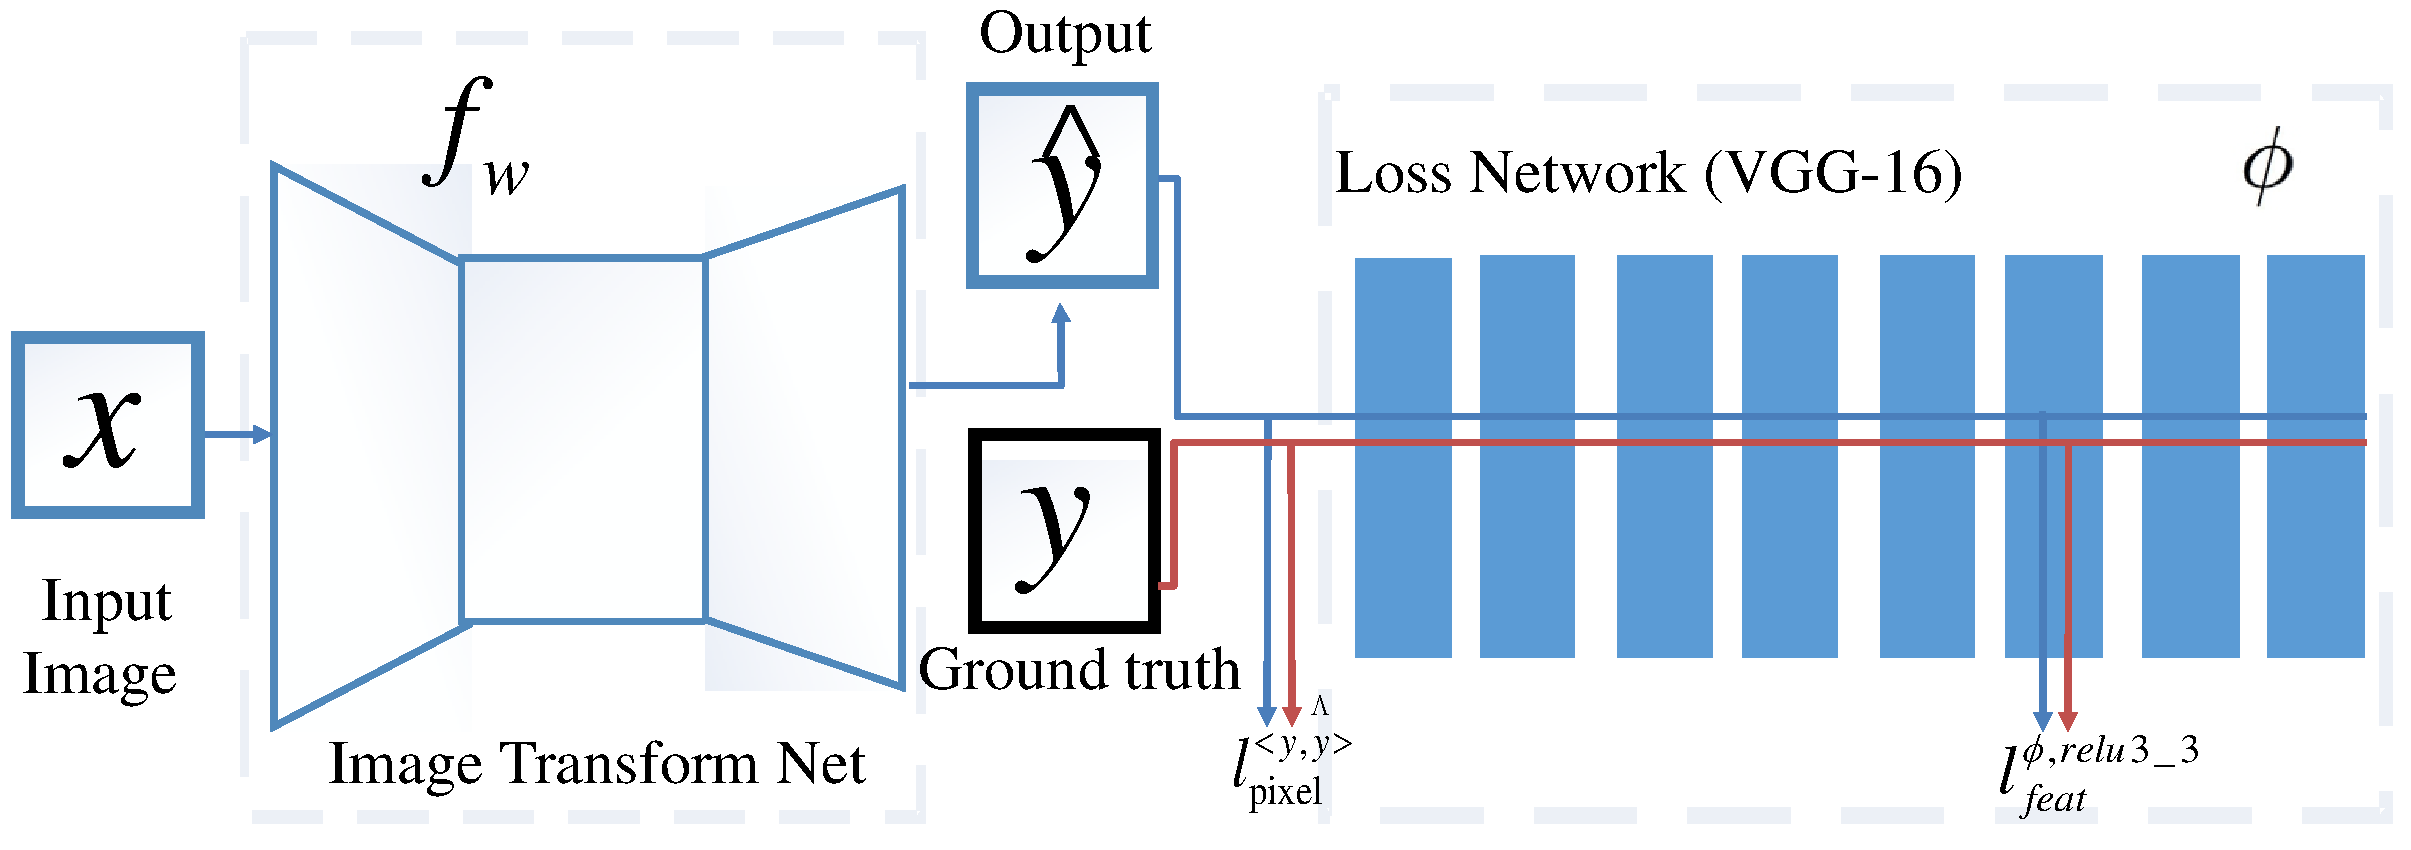
\includegraphics[width=0.9\textwidth]{ch06_01}
\caption[提出网络的整体架构图]{我们提出的网络的整体架构。图像变换网络包含卷积(编码器)和解卷积(解码器)层。我们使用预先训练的图像分类的损失网络来定义感知损失函数,这些函数测量输出和地面真实标签的感知差异。损失网络在训练过程中保持不变。}
\label{fig:ch06_01}
\vspace{-10mm}
\end{figure*}
 
所提出的框架主要包含一系列卷积层和解卷积层,如图\ref{fig:ch06_01}所示。它由两部分组成:一个\emph {图像转换网络} $ f_W $和一个\emph{loss network} $ \phi $,用于定义几个\emph {丢失函数} $ \ell_1,\ldots,\ell_k$。旨在学习由权重$ W $参数化的深度剩余卷积神经网络; 它通过映射$ \hat y = f_W(x)$将输入图像$ x $转换成输出图像$ f_W $。
每个损失函数计算标量值$ \ell_i(\hat y,y_i)$,测量输出图像$ \hat y $和 \emph{target image} $ y_i $之间的差异。学习目标是使用随机梯度下降来训练以最小化损失函数的加权组合:
\begin{equation}
   W^* = \arg\min_W E_{x, \{y_i\}}\begin{bmatrix}
\sum_{i=1} \lambda_i \ell_i(f_W(x), y_i)
\end{bmatrix}
\end{equation}
从这个公式中,我们可以看到这里的任务是找到最接近图像变换的映射函数$ f_W $。同时我们也希望$ f_W(y_i)$近似于图像$ y_i $,所以我们现在通过在不同情况下选择合适的权重$ W $来将图像去噪问题统一在一个统一的框架中。损失网络$ \phi $用于定义一个\emph{特征空间损失} $ \ell_{feat}^\phi $和一个\emph{per-pixel loss} $ \ell_{mse} $,功能和图像空间。对于图像去噪,输入图像$ x $是一个有噪声的输入,地面实况图像$ y $也是输入图像和目标图像。
  
\begin{figure}[t]
\centering
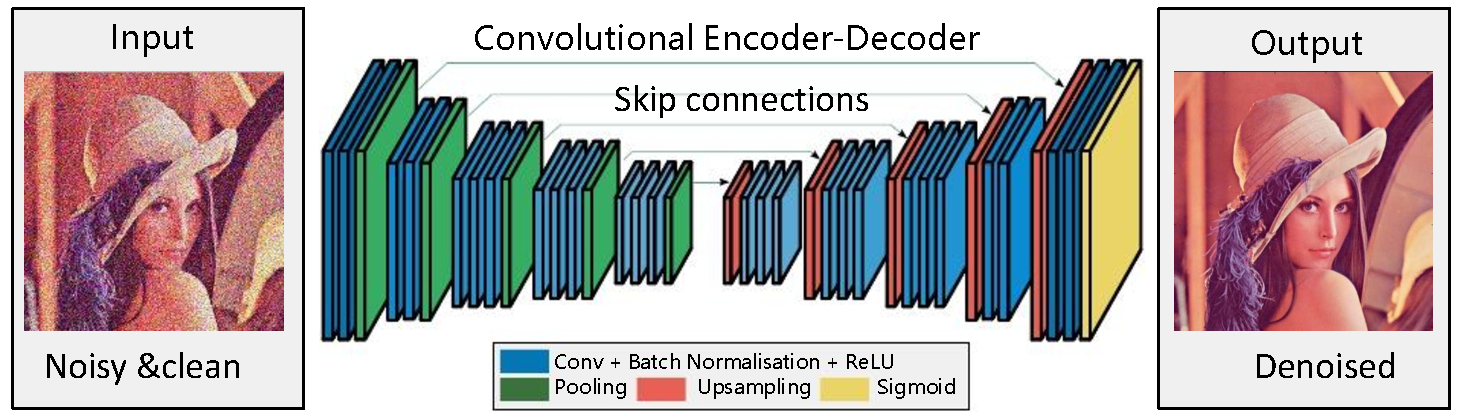
\includegraphics[width=0.9\textwidth]{ch06_02}
\caption{ RED-NET的网络结构图}
\label{fig:ch06_02}
\vspace{-6mm}
\end{figure} 
\subsubsection{编码器-解码器卷积结构}

该框架完全是编码器 - 解码器卷积模型。已经提出了用于无监督和有监督深度学习的编码器和解码器层的组合\cite{NohH2015,hong2015decoupled,Long2017Fully,Dong2016,Mao2016}。

我们的图像转换网络大致遵循\cite{Mao2016}提出的架构准则。他们提出RED-NET用于图像去噪,网络如图\ref{fig:ch06_02}所示。基于该网络结构,在卷积之后添加批量归一化\cite{Ioffe2014Batch}和ReLU非线性层。并在网络中插入一些残留块\cite{he15}。输出图层使用sigmoid函数来确保输出图像的像素范围为[0,1]。但是我们不使用任何汇聚层,而是使用分步和分步的卷积来进行下采样和上采样。除了使用9 $ \times $ 9内核的第一层和最后一层之外,所有卷积层都使用3 $ \times $ 3内核。由于图像变换网络是完全卷积的,因此在测试时它们可以应用于任何尺寸的图像。

RED-NET和我们的DeNET的区别在于我们的网络插入了一些残留块并引入了剩余连接。噪声在每层之后逐步消除。在此过程中,图像内容的细节可以通过感知丢失函数进行补偿。两个网络的具体配置在表 \ref{table1}中描述。

将两种学习策略应用于编解码网络的内部块,以使训练更有效。跳过连接每两个卷积层传递到它们的镜像解卷积层。He 等\cite{he15}使用剩余连接来训练非常深的网络进行图像分类。他们认为,剩余连接使网络很容易学习识别功能;这对于图像变换网络来说是一个吸引人的特性,因为在大多数情况下,输出图像应该与输入图像共享结构。因此,我们网络的主体由多个残余块组成,每个残块包含两个3 $ \times $ 3卷积层
 
\begin{table}
\vspace{-4mm}
\centering
\caption[DeNET-R和RED-NET网络的配置参数表]{DeNET-R和RED-NET网络的配置。“conv3”和“deconv3”代表大小为$ 3 \times3 $的卷积和反卷积内核。32,128和512是每个卷积和反卷积之后的特征映射的数量。“$ c $”是输入和输出图像的通道数量。即$ c = 3 $。}
\begin{tabular}{l | l }\hline
DeNET-R                   &RED-NET                \\ \hline
(conv9-32)$\times$6             &(conv3-128)$\times$6       \\ \hline
(conv3-64)$\times$6             &(conv3-256)$\times$6       \\ \hline
(conv3-128)$\times$3             &(conv3-512)$\times$3       \\ \hline
Residual block$\times$5 &                           \\ \hline
(deconv3-64)$\times$2           &(deconv3-512)$\times$2       \\ \hline
(deconv3-32)$\times$6           &(deconv3-512)$\times$6       \\ \hline
(deconv9-3) $\times$6           &(deconv3-512)$\times$6       \\ \hline
(deconv3-$c$)           &(deconv3-$c$)                \\ \hline
\end{tabular}
\label{table1}
%\vspace{-15mm}
\end{table}
\subsubsection{像素损失函数}
\emph{像素丢失}是输出图像之间的(归一化)欧几里德距离$ \hat y $和目标$ y $。如果两者都形成了$ C \times H \times W $,那么像素欧几里得损失就是
定义为均方误差(MSE):
 \begin{equation}
   \ell_2(\hat y, y) = \frac{1}{CHW}\|\hat y - y\|_2^2
  \end{equation}


这种损失函数可能会引入splotchy文物,因此我们也检查了\lone-norm损失。这两种损失对错误的权衡是不同的:\lone 不会过度惩罚更大的错误,因此它们可能具有不同的收敛性质。计算单独损失很简单:
\begin{equation}
\ell_1(\hat y, y) = \frac{1}{CHW}| \hat y - y|
\end{equation}
The derivatives for the back-propagation are also simple,  for each pixel $p$ in the whole image,
\begin{equation}
\partial \ell_1/\partial p  = sign\left(\hat y(p) - y(p)\right)
\end{equation}
请注意,虽然在整个图像上计算$ L_{\ell_1} $,则导数将针对图像中的每个像素进行反向传播。用 训练的网络为上述几个问题提供了重大改进。

\subsubsection{感知损失函数}

我们定义了测量图像之间感知和语义差异的\emph{感知损失函数},而不是\cite{Zhao2015}中的手工设计SSIM损失。他们利用\emph{loss network} $ \phi $ pretrained用于图像分类。在我们所有的实验中,$ \phi $都是16层VGG网络\cite{Simonyan2014a}在ImageNet数据集\cite{Deng2009ImageNet}上预训练。
而不是鼓励输出图像$ \hat y = f_W(x)$的像素完全匹配目标图像$ y $的像素,我们反而鼓励它们具有相似的特征表示由损失网络$ \phi $计算。让$ \phi_j(x)$为激活处理图像$ x $时的$ j $ th层网络$ \phi $; 如果$ j $是卷积层然后$ \phi_j(x)$将是形状的特征映射$ C_j \times H_j \times W_j $。\emph {feature feat loss}是特征表示之间的(平方,归一化)欧几里得距离: 
\begin{equation}
  \ell_{feat}^{\phi,j}(\hat y, y) = 
  \frac1{C_jH_jW_j}\|\phi_j(\hat y) - \phi_j(y)\|_2^2
\end{equation}
欧几里德距离也可以交替$ \ell_{1} $ - 范数距离。如\cite{Mahendran2015}所示,找到一个图像$ \hat y $,以最小化该特征
早期图层的专长往往会产生与$ y $无法区分的图像。鼓励使用特征专长丢失来训练我们的图像转换网络输出图像$ \hat y $与感兴趣的图像$ y $相似,但不会强制它们完全匹配。为了鼓励输出图像$ \hat y $的空间平滑度,我们请遵循之前关于功能反转\cite{Mahendran2015}的工作,并使用\emph {总变化正则化函数} $ \ell_{TV}(\hat y)$。
 
\subsection{实验结果分析和讨论}
\label{sec:experiments-results}

在本节中,我们用完全编码器 - 解码器卷积神经网络对我们的实验设置进行分析。然后评估我们的模型在一些不同的损耗函数设置下的去噪性能。最后,我们探讨如何让一个神经网络处理不同程度的噪音。
\subsection{详尽分析模型}

\begin{table}[b]\label{tab:Denoising-results}  
\vspace{-2mm} 
\footnotesize% fontsize
   \centering{
   \caption{{\it Set14}上的定量单级图像去噪结果表}
   \scalebox{0.75}{
     \begin{tabular}{|c|c|c|c|c|c|c|}
       \hline
        \multirow{2}{*}{Sigma} & Noisy & RED-NET\cite{Mao2016} & Ours ($\ell_{2})$ & Ours ($\ell_{1}$)& Ours ($\ell_{feat}$) & Ours ($\ell_{mix}$)\\
   & PSNR / SSIM & PSNR / SSIM & PSNR / SSIM & PSNR / SSIM & PSNR / SSIM & PSNR / SSIM\\
   \hline
    \multirow{1}{*}{$\sigma=10$} & 28.16 / 0.7041 & \textbf{34.81} / \textbf{0.9402}
           & 34.35 / 0.8912 & 33.40 / 0.8930& 31.05 / 0.7680& 33.16 / 0.7680  \\
          % \hline 
    \multirow{1}{*}{$\sigma=30$} & 18.88 / 0.3389 & 29.17 / 0.8423
           & 28.73 / 0.8205 & 29.76 / 0.991& 26.70 / 0.6845& \textbf{30.15} / \textbf{0.8681}  \\
          % \hline
    \multirow{1}{*}{$\sigma=50$} & 14.79 / 0.2038 & 26.81 / 0.7733
           & 26.40 / 0.8205 & 26.79 / \textbf{0.8325}& 25.69 / 0.6411& \textbf{27.09} / 0.8312  \\
          % \hline
    \multirow{1}{*}{$\sigma=70$} & 12.43 / 0.1391 & 25.31 / 0.7206
           & 25.39 / 0.7105 & 26.13 / \textbf{0.7250}& 17.89 / 0.6650& \textbf{26.20} / 0.7180  \\
    \multirow{1}{*}{$\sigma=100$} & 10.26 / 0.0901 &  -
           & 18.40 / 0.4215 & 20.17 / 0.4680& 17.31 / 0.3640& \textbf{19.16} / \textbf{0.4695}  \\
           \hline
        
\end{tabular} 
}}  
\vspace{-4mm}
\end{table}
我们通过最小化一些损失函数来训练模型执行单个和多个标准偏差$ \sigma $:$ \ell_{2} $ - 均方误差(MSE)损失,$ \ell_{1} $ - 范数损失和特征在
图层上的壮举损失。从VGG-16网络$ \phi $。我们用训练集中的$ 256 \times 256 $训练图像大小,并通过添加宽度为$ \sigma $的高斯内核来准备噪声输入。我们使用Adam\cite{Kingma2014Adam}以10美元的批次大小进行训练,学习速度为$1 \times 10^{-3}$美元,没有减重或辍学。

去噪实验在标准的14个通用基准图像{\it Set14}上执行。作为文献中常见的实验设置,将零均值和标准差$ \sigma $的加性高斯噪声添加到测试图像中,以测试去噪方法的性能。我们报告PSNR和SSIM\cite{Wang2004},计算两个三通道彩色图像,参考文献\citep{Mao2016,Zhao2015}。

作为基准模型,我们使用RED-NET\cite{Mao2016}提供最先进的性能。它是一个完全卷积网络,具有卷积和去卷积层以减少每像素损失。为了说明RED-NET和我们的模型在数据,训练和网络结构方面的差异,我们使用$ \ell_{2} $对相同的标准偏差$ \sigma $进行图像变换网络训练;这些网络使用与经过训练的网络相同的数据,网络结构和训练,以尽量减少其他损失功能。我们使用通常使用的每像素丢失来对去噪网络进行训练,这些网络同样带有特征专长丢失(见Section\ref{sec:method}),以允许从预训损失网络传输语义知识作为有监督的信号指导去噪的去噪网络。

\begin{figure}[t]
\centering
  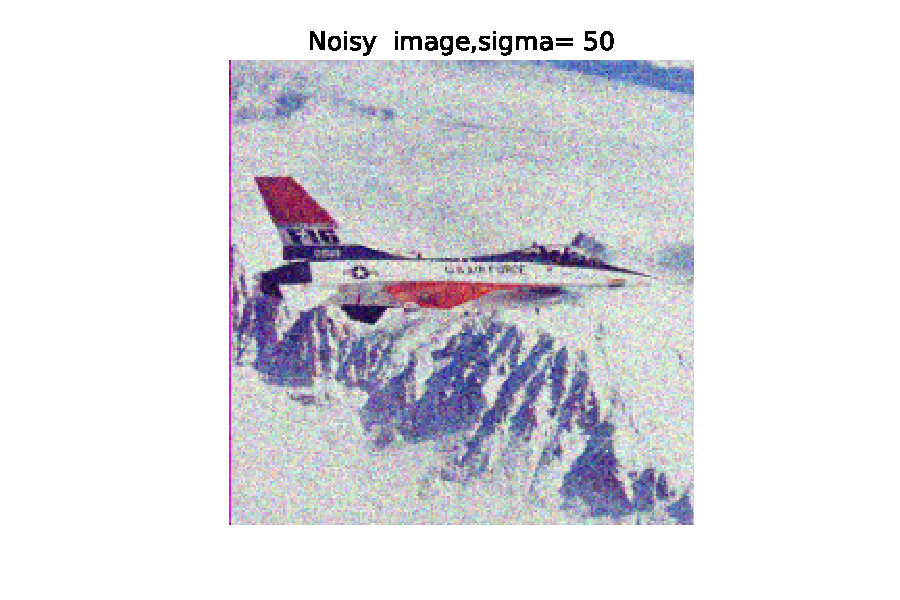
\includegraphics[width=0.17\textwidth]{figs/loss/noisy.pdf}
  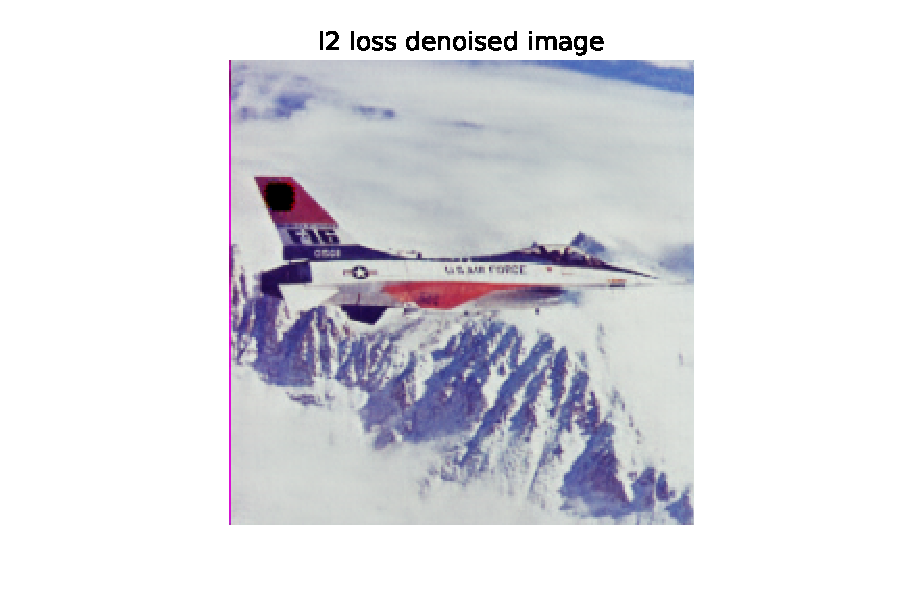
\includegraphics[width=0.17\textwidth]{figs/loss/l2.pdf}
  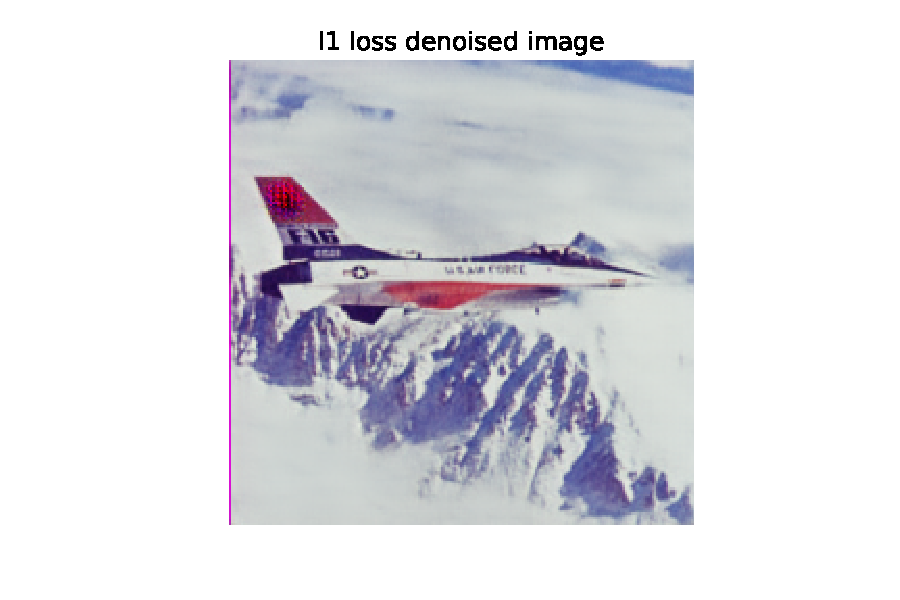
\includegraphics[width=0.17\textwidth]{figs/loss/l1.pdf}
  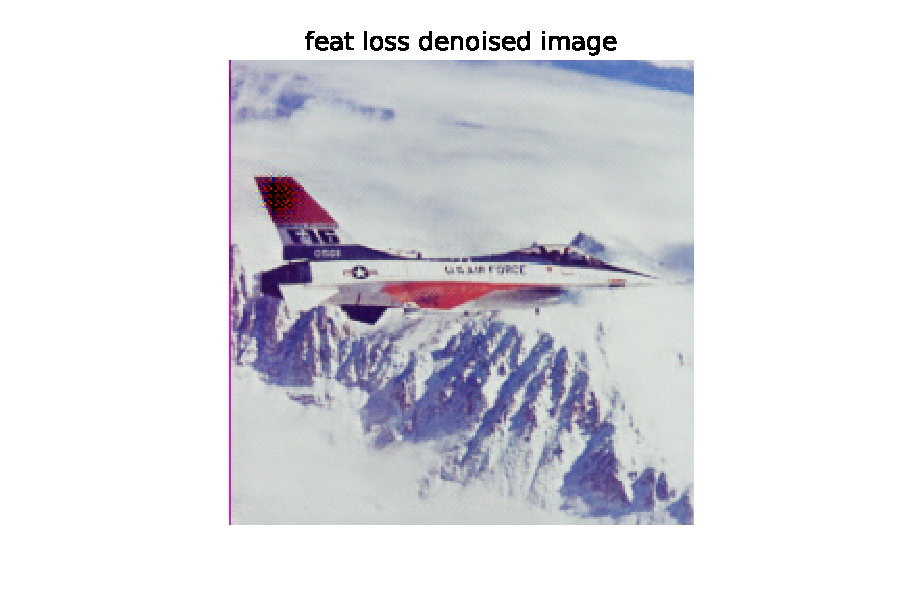
\includegraphics[width=0.17\textwidth]{figs/loss/feat.pdf}
  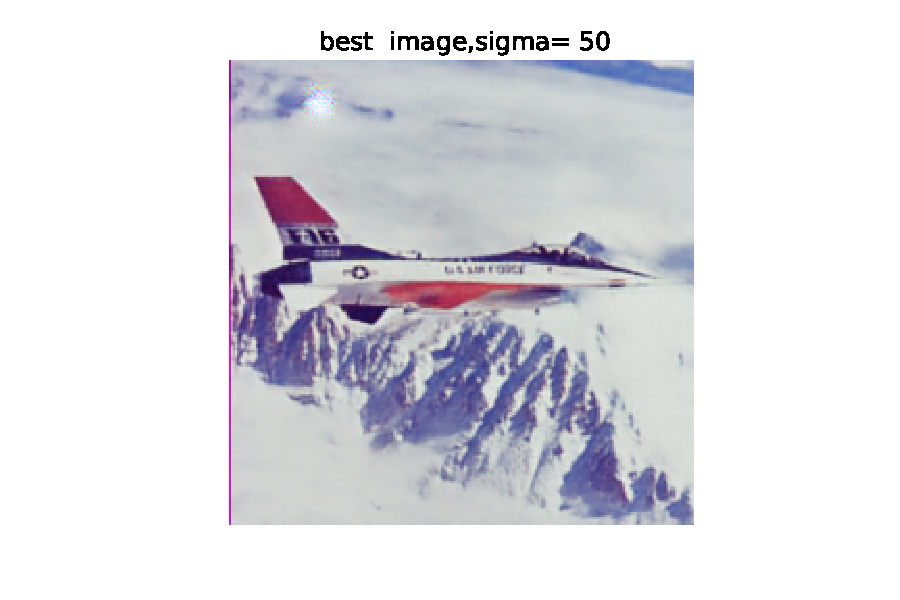
\includegraphics[width=0.17\textwidth]{figs/loss/mix.pdf}  \\{}
  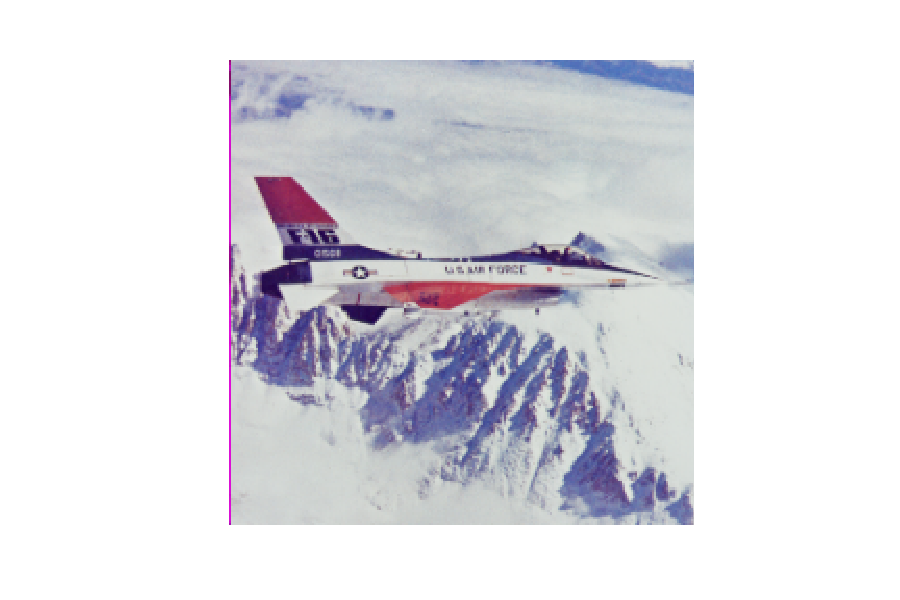
\includegraphics[trim={15pt 60pt 15pt 62pt},width=0.17\textwidth,clip]{figs/loss/orign.pdf}
  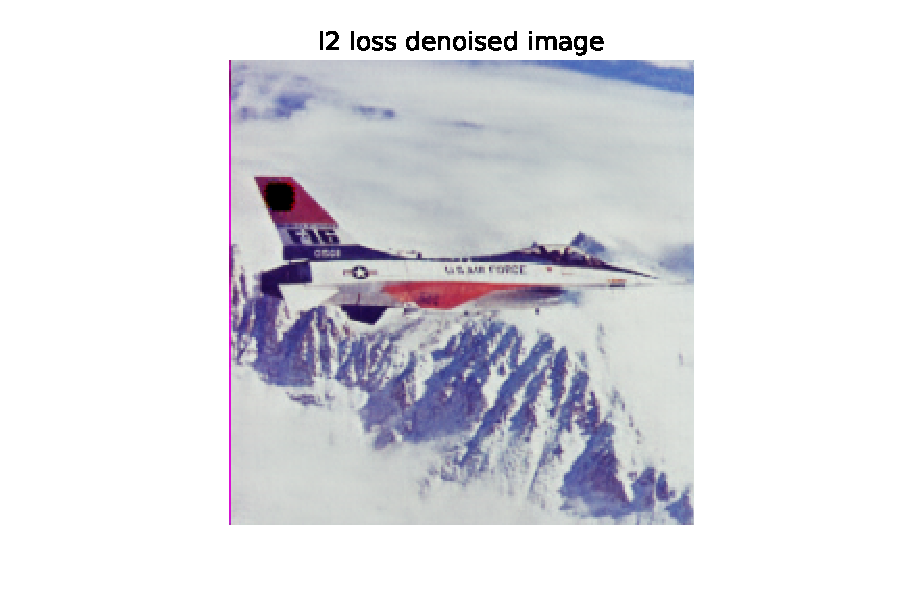
\includegraphics[trim={15pt 60pt 15pt 75pt},width=0.17\textwidth,clip]{figs/loss/l2.pdf}
  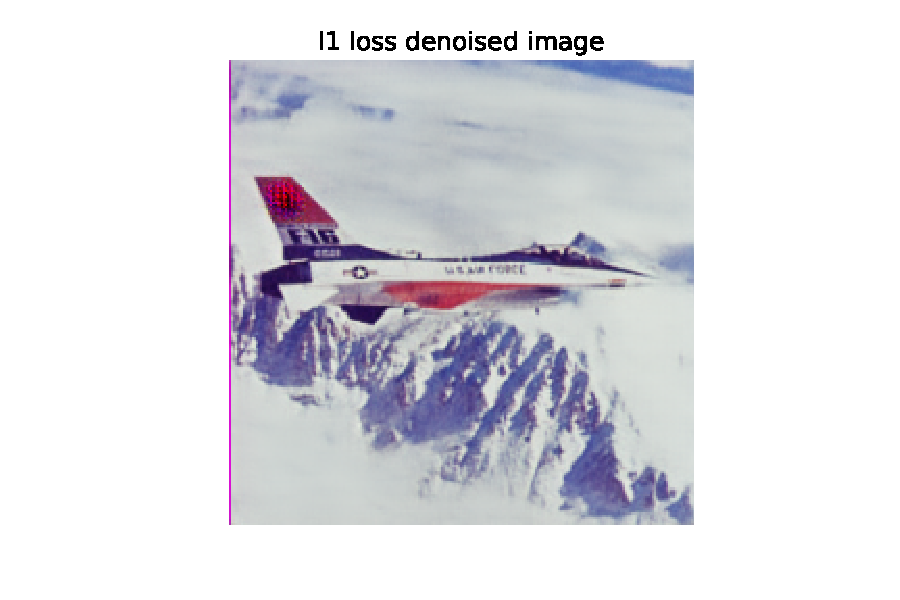
\includegraphics[trim={15pt 60pt 15pt 75pt},width=0.17\textwidth,clip]{figs/loss/l1.pdf}
  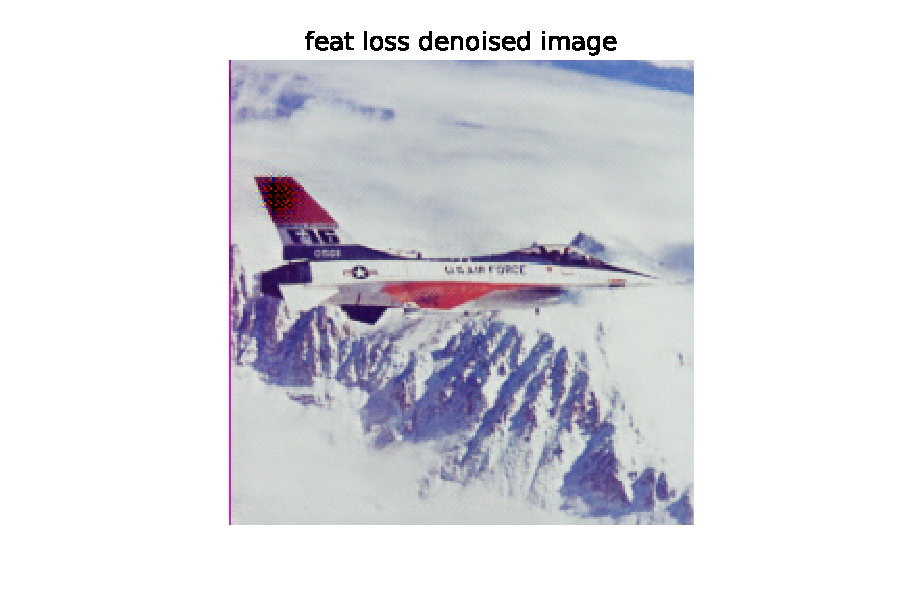
\includegraphics[trim={15pt 60pt 15pt 75pt},width=0.17\textwidth,clip]{figs/loss/feat.pdf}
  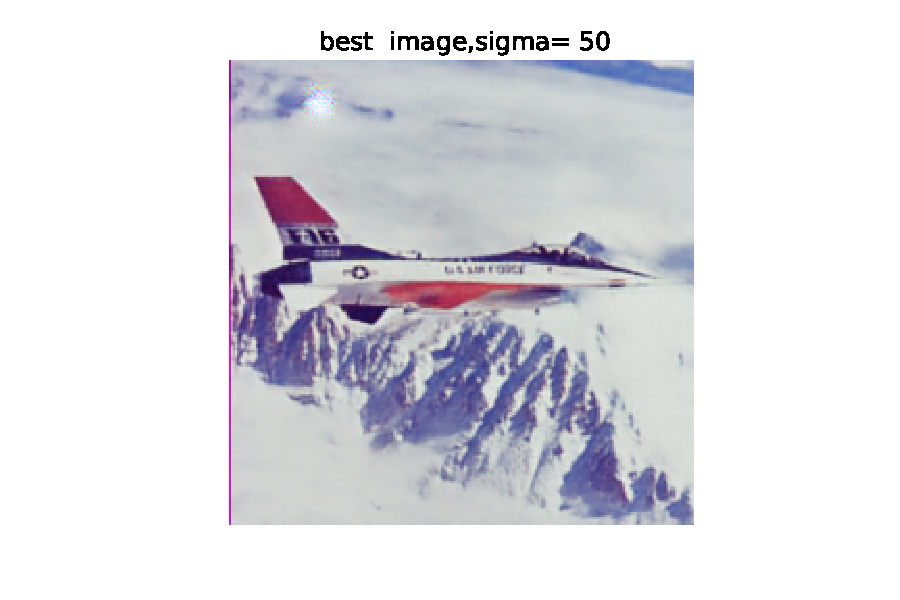
\includegraphics[trim={15pt 60pt 15pt 75pt},width=0.17\textwidth,clip]{figs/loss/mix.pdf} \\
   \begin{minipage}{0.17\textwidth}
        \centering \textbf{Ground Truth} \\ PSNR / SSIM
   \end{minipage}
   \begin{minipage}{0.17\textwidth}
     \centering \textbf{Ours}($\ell_{2}$) \\ 29.11 / 0.8833
   \end{minipage}
   \begin{minipage}{0.17\textwidth}
     \centering \textbf{Ours} ($\ell_{1}$) \\ 29.27 / 0.8841
   \end{minipage}
   \begin{minipage}{0.17\textwidth}
     \centering \textbf{Ours} ($\ell_{feat}$) \\  19.61 / 0.6560
   \end{minipage}
   \begin{minipage}{0.17\textwidth}
     \centering \textbf{Ours} ($\ell_{mix}$) \\  29.31 / 0.8946
   \end{minipage} \\
  \caption[不同损失在基准数据库上的定量比较结果表]{不同损失在基准数据库上的定量比较结果表,在来自{\it Set14}数据集的图像上以不同的损失类型去噪结果。 我们以F-16图像报告PSNR / SSIM为例。 
  }
  \vspace{-4mm}
  \label{fig:l1-l2-feat-results}
\end{figure}
首先,与每像素损失$ \ell_{1} $和$ \ell_{2} $结果相比,$ \ell_{1} $在去噪性能方面做得更好,同时还原了锐利的边缘和细节细节。如图\ref{fig:l1-l2-feat-results}所示
$ \ell_{2} $图像中的机翼以及$ \ell_{2} $图像中的主体的红色块元素。这是因为$ \ell_{2} $惩罚更大的错误,但更宽容无论图像中的底层结构如何,都会产生小的错误;结论与文献{Zhao2015}一致。

此外,只有当特征专长丢失时,在放大倍数下才能看到轻微的交叉影线模式,结果为$ \ell_{feat} $显示在图\ref{fig:l1-l2-feat-results}与基线方法相比,会损害其PSNR和SSIM。我们再次看到,与其他模型相比,我们的$ \ell_{feat} $模型在边缘和细节方面做得很好,比如机翼。$ \ell_{feat} $模型不会不加区分地锐化;与$ \ell_{pixel} $模型相比,$ \ell_{feat} $模型锐化了机翼和骑手的边界边缘,但背景山仍然是漫反射的,这表明$ \ell_{feat} $模型可能是更了解图像语义。

由于我们的$ \ell_{pixel} $和$ \ell_{feat} $模型共享相同的架构,数据和训练过程,它们之间的所有差异都是由于$ \ell_{pixel} $和$ \ell_{feat} $损失。$ \ell_{pixel} $损失产生较少的视觉伪像和较高的PSNR值,但$ \ell_{feat} $损失在重建细节方面做得更好,从而导致令人满意的视觉效果。

最后,我们可以观察到单个模型可以在所有级别的高斯噪声中工作,从而允许显着减少通用神经网络驱动的去噪算法的训练时间。原因可能是学习图像变换函数可以从任何级别和其他类型对高斯分布进行建模。有趣的是,如图\ref{fig:other-type-results}所示,即使对于其他类型的噪声,如模型为高斯噪声训练的斑点噪声,分布式噪声,盐噪声或胡椒噪声等,也具有图像去噪的能力。

\begin{figure}[t]
 \centering
   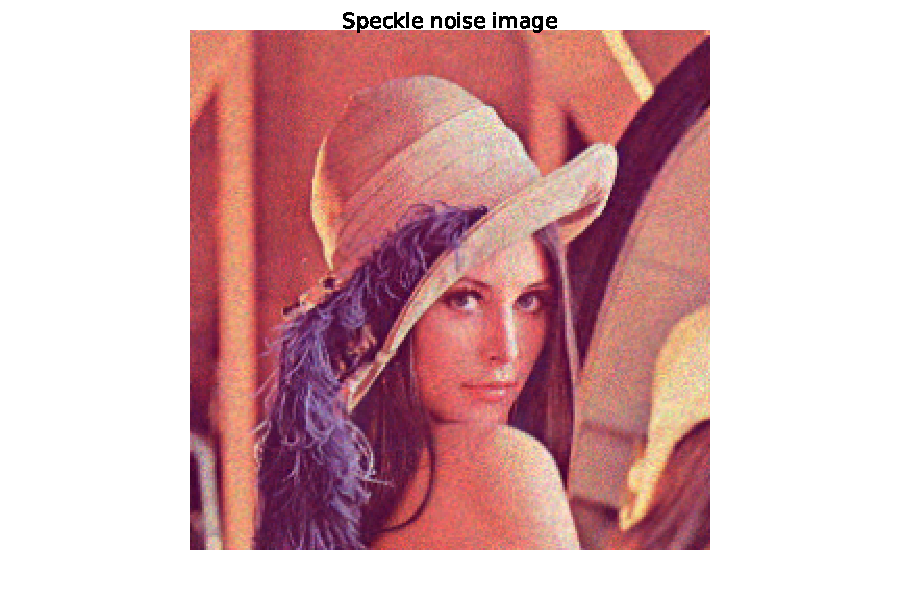
\includegraphics[width=0.24\textwidth]{figs/speckle}
  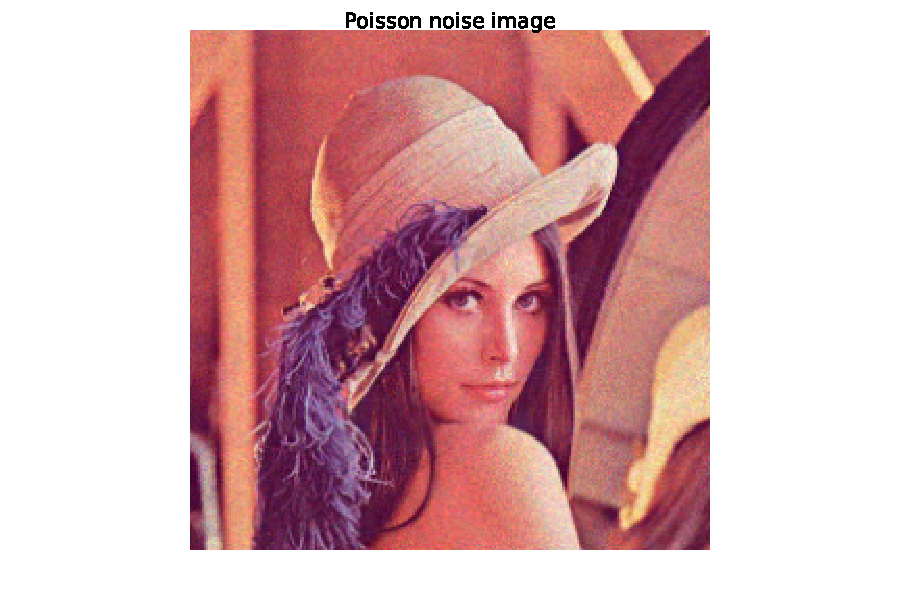
\includegraphics[width=0.24\textwidth]{figs/poisson}
  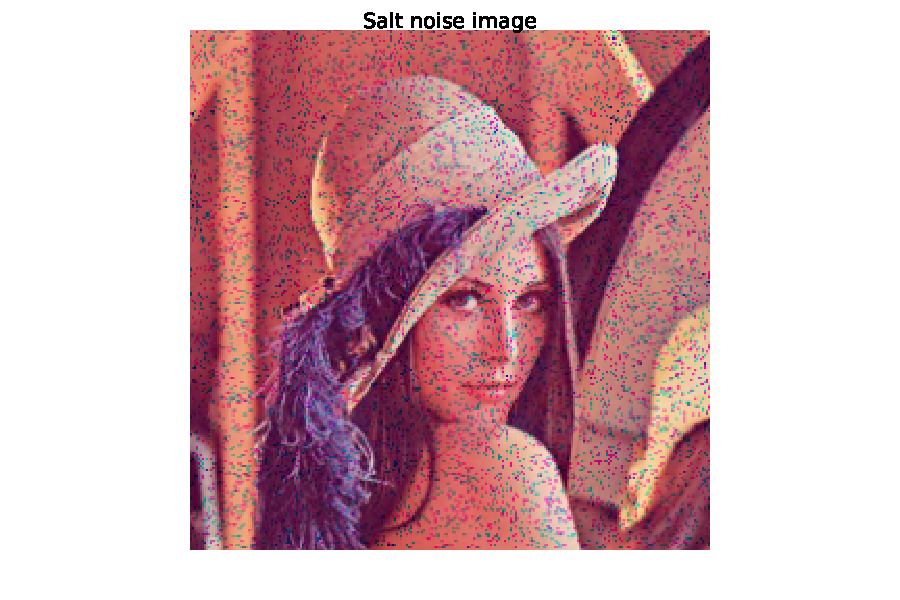
\includegraphics[width=0.24\textwidth]{figs/salt}
  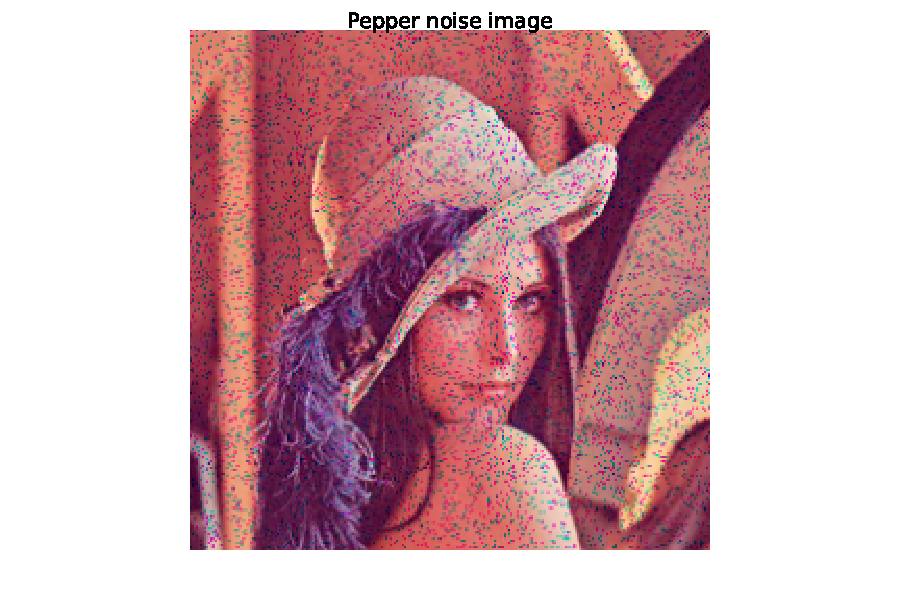
\includegraphics[width=0.24\textwidth]{figs/pepper} \\{}
  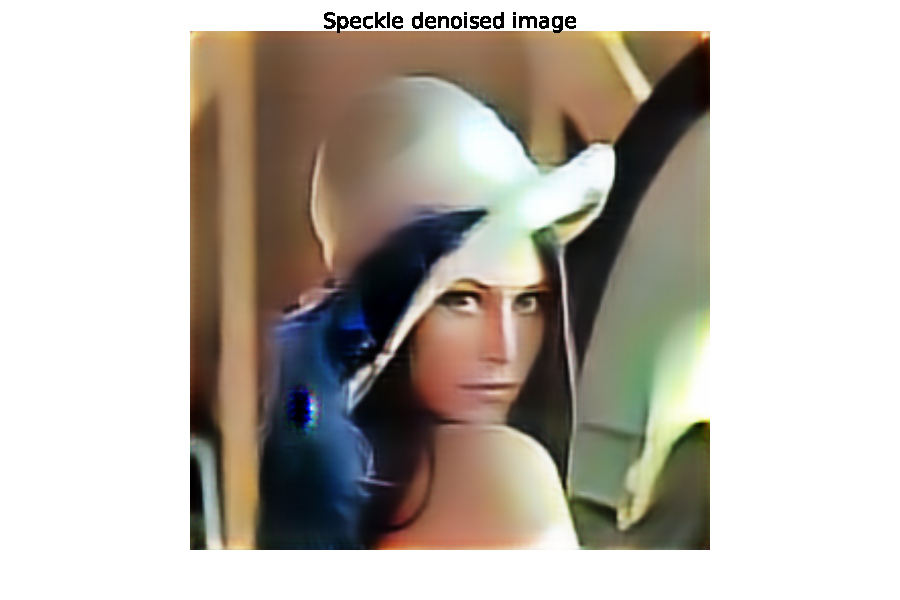
\includegraphics[trim={160pt 30pt 150pt 200pt},width=0.24\textwidth,clip]{figs/speckle_denoised}
  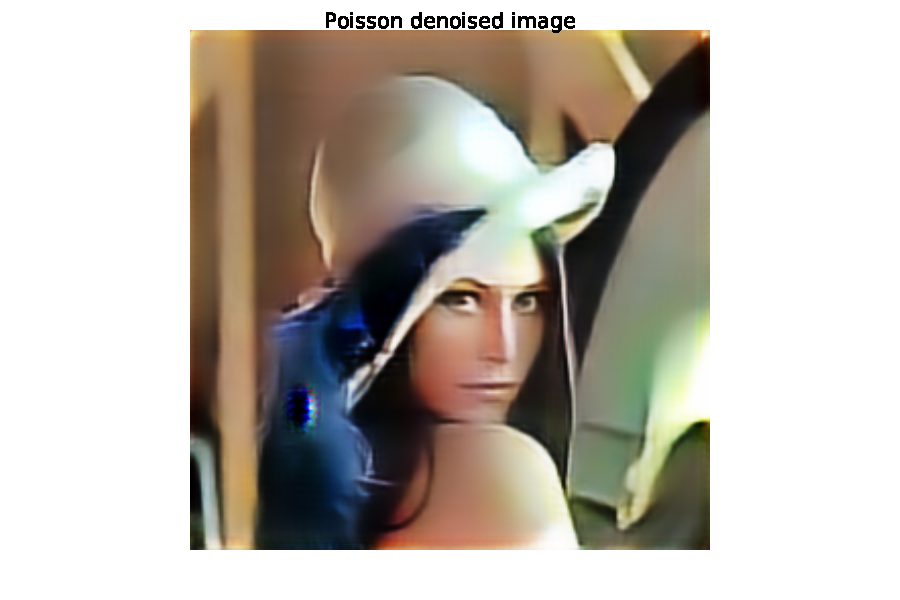
\includegraphics[trim={160pt 30pt 150pt 200pt},width=0.24\textwidth,clip]{figs/poisson_denoised}
  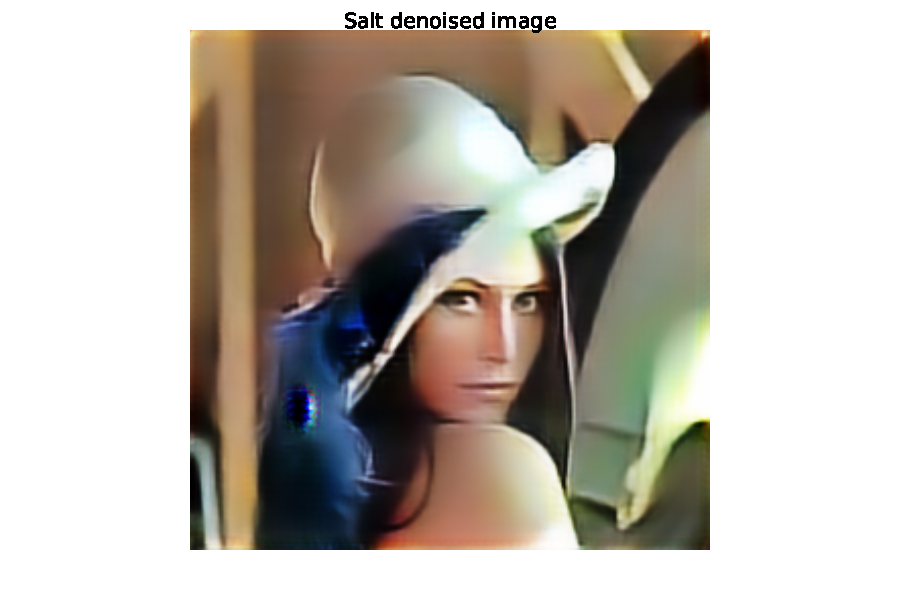
\includegraphics[trim={160pt 30pt 150pt 200pt},width=0.24\textwidth,clip]{figs/salt_denoised}
  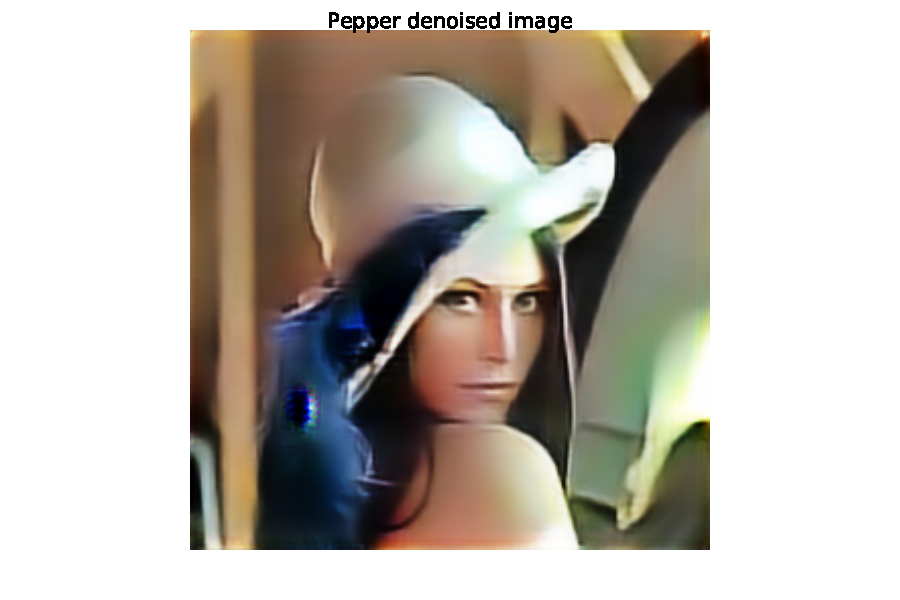
\includegraphics[trim={160pt 30pt 150pt 200pt},width=0.24\textwidth,clip]{figs/pepper_denoised} \\
    
   \caption[四种其他噪声类型的比较去噪结果图]{四种其他噪声类型的比较去噪性能,其中转换网络仅用高斯噪声进行训练。\textbf{Up:}四种类型的噪声图像:散斑噪声,泊松分布噪声,盐噪声,胡椒噪声。\textbf{Down:}从相应的噪声类型中去噪子输出。
   }
   \vspace{-4mm}
   \label{fig:other-type-results}
 \end{figure}
 
